\documentclass[conference]{IEEEtran}
\usepackage[utf8]{inputenc}
\usepackage{graphicx}
\usepackage{amsmath}
\usepackage{cite}
\usepackage{float}

\title{Migración en El Salvador: Una Perspectiva Socioeconómica}
\author{\IEEEauthorblockN{Natanael de Jesús Rivera Hernández}
\IEEEauthorblockA{Facultad de ingenieria\\
Universidad Francisco  Gavidia\\
Email: natanael.rivera@gmail.com}
\and
\IEEEauthorblockN{Rene Salvador Cardoza Godínez}
\IEEEauthorblockA{Facultad de ingenieria\\
Universidad Francisco Gavidia\\
Email: rene.cardoza@gmail.com}
}

\begin{document}
\maketitle

\begin{abstract}
    La migración en El Salvador ha representado un fenómeno de gran importancia que ha moldeado profundamente su desarrollo en aspectos sociales, económicos y políticos. Este artículo se centra en examinar, de manera detallada, las diversas causas que impulsan a las personas a migrar desde El Salvador hacia otros países, explorando factores como la falta de oportunidades económicas, la violencia, la inestabilidad política y los vínculos familiares en el extranjero. Asimismo, se analizan las repercusiones que este fenómeno tiene en la sociedad salvadoreña, destacando sus efectos tanto positivos como negativos en áreas clave como la economía, mediante las remesas, y el tejido social, debido a la fragmentación familiar.

    El texto también presenta un enfoque sobre las posibles soluciones para abordar los desafíos que la migración plantea, incluyendo estrategias para mitigar sus consecuencias negativas y maximizar los beneficios potenciales. Se proponen medidas que abarcan desde políticas públicas orientadas a mejorar las condiciones de vida en el país hasta iniciativas para apoyar a los migrantes y sus familias en el extranjero. Además, se incorporan datos estadísticos relevantes, representaciones gráficas e incluso fórmulas matemáticas que respaldan y enriquecen el análisis presentado, ofreciendo una perspectiva integral sobre este fenómeno y sus múltiples dimensiones.
\end{abstract}

\section{Introducción}
La migración ha sido un fenómeno constante en El Salvador, influenciado por factores como la violencia, la falta de oportunidades económicas y los desastres naturales. Según estudios recientes \cite{unmigration2021}, un porcentaje significativo de la población salvadoreña reside en el extranjero, principalmente en los Estados Unidos.

\section{Causas de la Migración}
Entre las principales causas de la migración en El Salvador se encuentran:
\begin{itemize}
    \item La violencia de las pandillas.
    \item La pobreza y el desempleo.
    \item Los desastres naturales como huracanes y terremotos.
\end{itemize}

\section{Impacto Socioeconómico}
La migración genera tanto efectos positivos como negativos en la economía de El Salvador, desempeñando un papel crucial en el desarrollo económico del país. Por un lado, las remesas enviadas por los salvadoreños en el exterior representan una fuente importante de ingresos para numerosas familias, contribuyendo significativamente al consumo interno y al crecimiento económico. Por otro lado, la pérdida de población activa debido a la emigración puede limitar el desarrollo del mercado laboral y afectar la capacidad productiva del país.

En este contexto, se incluyen dos tablas que presentan datos detallados sobre las remesas enviadas desde el extranjero y la distribución de la población migrante salvadoreña. Estas tablas permiten visualizar el impacto económico de las remesas en términos de su contribución al Producto Interno Bruto (PIB), así como identificar las características demográficas y los destinos principales de los migrantes. Los datos aportados ofrecen una visión más profunda y cuantitativa de cómo la migración influye en la economía del país, destacando tanto sus beneficios como los desafíos asociados.
\subsection{Tabla de Remesas Recibidas}
\begin{table}[H]
\caption{Remesas recibidas en El Salvador (2020-2023).}
\label{table_remesas}
\centering
\begin{tabular}{|c|c|c|}
\hline
Año & Remesas (millones de \$) & Variación (\%) \\ \hline
2020 & 5700 & -5.0 \\ \hline
2021 & 6500 & 14.0 \\ \hline
2022 & 7000 & 7.7 \\ \hline
2023 & 7300 & 4.3 \\ \hline
\end{tabular}
\end{table}

\subsection{Distribución de Migrantes}
\begin{table}[H]
\caption{Distribución de migrantes salvadoreños por región.}
\label{table_migrantes}
\centering
\begin{tabular}{|l|c|}
\hline
Región & Porcentaje (\%) \\ \hline
América del Norte & 85 \\ \hline
América Latina & 10 \\ \hline
Europa & 4 \\ \hline
Asia y Oceanía & 1 \\ \hline
\end{tabular}
\end{table}

\section{Análisis Matemático}
Se pueden modelar las remesas recibidas utilizando una progresión geométrica:
\begin{equation}
R_n = R_0 \cdot (1 + g)^n, \quad \text{donde } g = \text{tasa de crecimiento}.
\label{eq:remesas}
\end{equation}

Además, la distribución de migrantes puede representarse por un sistema de ecuaciones para las distintas regiones:
\begin{equation}
P_{\text{total}} = P_{\text{América del Norte}} + P_{\text{América Latina}} + P_{\text{Europa}} + P_{\text{Asia y Oceanía}}.
\label{eq:distribucion}
\end{equation}

\section{Representación Visual}
\subsection{Imágenes de Apoyo}
En la Figura~\ref{fig:migrantes}, se presenta un gráfico que ilustra las rutas migratorias más comunes desde El Salvador.

\begin{figure}[H]
\centering
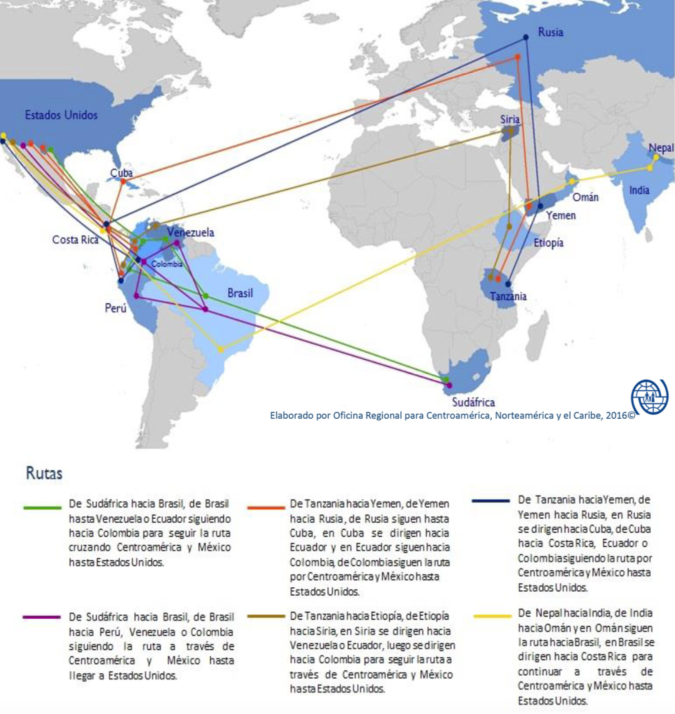
\includegraphics[width=0.45\textwidth]{imagenes/rutas_migratorias.png}
\caption{Rutas migratorias desde El Salvador.}
\label{fig:migrantes}
\end{figure}

\subsection{Imagen a Dos Columnas}
\begin{figure*}[t]
\centering

\includegraphics[width=\textwidth]{imagenes/impacto_remesas.png}
\caption{Impacto de las remesas en la economía salvadoreña.}
\label{fig:remesas}
\end{figure*}

\section{Conclusión}
En conclusión, la migración en El Salvador constituye un fenómeno multidimensional y profundamente arraigado en desafíos estructurales como la pobreza, la violencia y la falta de oportunidades. No obstante, con la implementación de políticas públicas bien diseñadas y estrategias integrales, es posible transformar este fenómeno en una oportunidad para el desarrollo sostenible. Aprovechar al máximo los beneficios económicos, sociales y culturales que aporta la diáspora salvadoreña, al tiempo que se mitigan los efectos negativos, requiere un enfoque coordinado que abarque tanto la mejora de las condiciones internas del país como el fortalecimiento de los vínculos con la población migrante en el exterior.
\section*{Agradecimientos}
Queremos expresar nuestro más sincero agradecimiento a la Universidad Francisco Gavidia por su valioso apoyo y colaboración en la realización de este estudio. Su respaldo fue fundamental para el desarrollo de este trabajo y para alcanzar los objetivos propuestos, reafirmando su compromiso con la generación de conocimiento y el impulso a la investigación académica en beneficio de la sociedad.

\bibliographystyle{IEEEtran}
\bibliography{referencias}

\end{document}